\documentclass[dutch]{ucll-slides}
\usepackage{pxfonts}
\usepackage{tikz}
\usepackage{calc}
\usepackage{ucll-code}


\usetikzlibrary{calc,shadows,tikzmark}

\coursename{Scripttalen}
\title{Hashing}



\begin{document}

\maketitle

\begin{frame}
  \frametitle{Premisse}
  \begin{itemize}
    \item Je bewaakt toegang tot een gebouw
    \item Je hebt een lijst namen
    \item Enkel mensen op de lijst mogen binnen
    \item Dit moet zo effici\"ent mogelijk gebeuren
  \end{itemize}
\end{frame}

\begin{frame}
  \frametitle{Poging \#1}
  \begin{center}
    \begin{tabular}{rl}
      $\square$ & Jan \\
      $\square$ & Pieter \\
      $\square$ & Dorien \\
      $\square$ & Eric \\
    \end{tabular}
  \end{center}
  \begin{itemize}
    \item Namen in random volgorde
    \item Ok indien klein aantal namen
  \end{itemize}
\end{frame}

\begin{frame}
  \frametitle{Lineair Zoeken}
  \begin{center}
    \begin{tabular}{cc}
      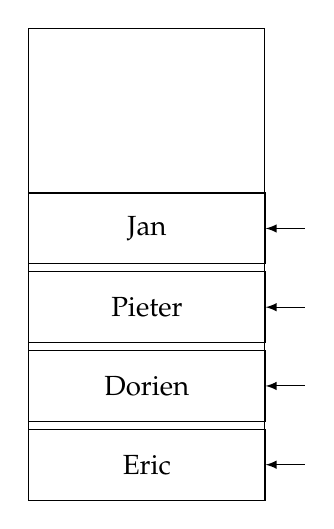
\begin{tikzpicture}
        \path[draw] (0,-4) rectangle (3,2);
        \foreach[count=\i] \name in {Jan,Pieter,Dorien,Eric} {
          \node[anchor=south west,draw,minimum width=3cm,minimum height=0.9cm] (name \i) at (0,-\i) {\name};
        }
        
        \foreach[evaluate={int(\i+1)} as \j] \i in {1,...,4} {
          \visible<\j>{
            \draw[latex-] (name \i.east) -- ++(0.5,0);
          }
        }
      \end{tikzpicture}
      
      \code[language=python,width=.5\linewidth]{linear-search.py}
    \end{tabular}
  \end{center}
  \begin{itemize}
    \item Zoeken naar 
  \end{itemize}
\end{frame}

\begin{frame}
  \frametitle{Verbetering}
  \begin{center}
    \begin{tabular}{rlrlrl}
      $\square$ & An      & $\square$ & Gunther   & $\square$ & Mieke \\
      $\square$ & Bart    & $\square$ & Hannelore & $\square$ & Nadia \\
      $\square$ & Dorien  & $\square$ & Idriss    & $\square$ & Patrick \\
      $\square$ & Eric    & $\square$ & Jolien    & $\square$ & Sanne \\
      $\square$ & Frans   & $\square$ & Karel     & $\square$ & Thomas \\
    \end{tabular}
  \end{center}
  \begin{itemize}
    \item Voor grotere aantallen is betere organisatie nodig
    \item Alfabetisch sorteren versnelt het proces
  \end{itemize}
\end{frame}


\end{document}



%%% Local Variables: 
%%% mode: latex
%%% TeX-master: t
%%% End: 
